\documentclass{article}

\usepackage{amsmath}
\usepackage{amsthm}
\usepackage{amssymb}
\usepackage{bm}
\usepackage{bbm}
\usepackage{fancyhdr}
% \usepackage{listings}
\usepackage{cite}
\usepackage{graphicx}
\usepackage{enumitem}
\usepackage{courier}
\usepackage[pdftex,colorlinks=true, urlcolor = blue]{hyperref}
\usepackage{pdfpages}


\oddsidemargin 0in \evensidemargin 0in
\topmargin -0.5in \headheight 0.25in \headsep 0.25in
\textwidth 6.5in \textheight 9in
\parskip 6pt \parindent 0in \footskip 20pt

% set the header up
\fancyhead{}
\fancyhead[L]{Stanford Aeronautics \& Astronautics}
\fancyhead[R]{Fall 2020}

%%%%%%%%%%%%%%%%%%%%%%%%%%
\renewcommand\headrulewidth{0.4pt}
\setlength\headheight{15pt}

\usepackage{xparse}
\NewDocumentCommand{\codeword}{v}{%
\texttt{\textcolor{blue}{#1}}%
}

\usepackage{xcolor}
\setlength{\parindent}{0in}

\title{AA 274A: Principles of Robot Autonomy I \\ Problem Set 2}
\author{Name: Li Quan Khoo     \\ SUID: lqkhoo (06154100)}
\date{\today}

\begin{document}

\maketitle
\pagestyle{fancy} 

\section*{Problem 1: Camera Calibration}
\begin{enumerate}[label=(\roman*)]
\item % (i)
(code)

\item % (ii)
(code)

\item % (iii)
(code)

\item % (iv)
(code)

\item % (v)
(code)

\end{enumerate}

\section*{Problem 2: Line Extraction}
\begin{enumerate}[label=(\roman*)]
\item % (i)
(code)

\item % (ii)

With parameters
\begin{enumerate}
	\item MIN\_SEG\_LENGTH = 0.05
	\item LINE\_POINT\_DIST\_THRESHOLD = 0.02
	\item MIN\_POINTS\_PER\_SEGMENT = 2
	\item MAX\_P2P\_DIST = 1
\end{enumerate}


\begin{tabular}[t]{l}
	\hline \\
	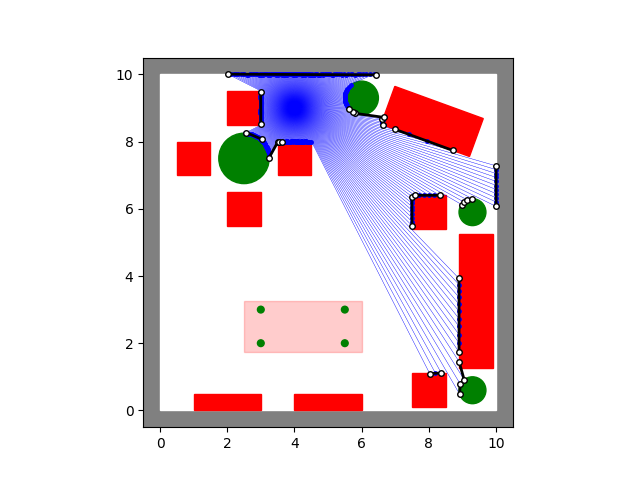
\includegraphics[width=0.80\textwidth]{img/rangeData_4_9_360.png} \\
	\hline
	Split-and-merge on \texttt{rangeData\_4\_9\_360} \\
\end{tabular}

\begin{tabular}[t]{l}
	\hline \\
	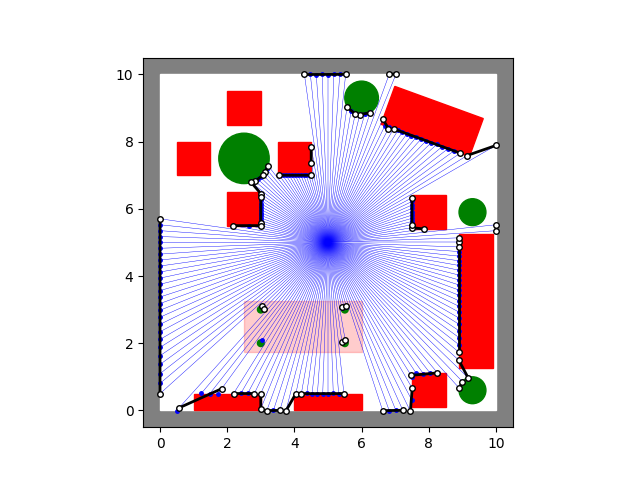
\includegraphics[width=0.80\textwidth]{img/rangeData_5_5_180.png} \\
	\hline
	Split-and-merge on \texttt{rangeData\_5\_5\_180} \\
\end{tabular}

\begin{tabular}[t]{l}
	\hline \\
	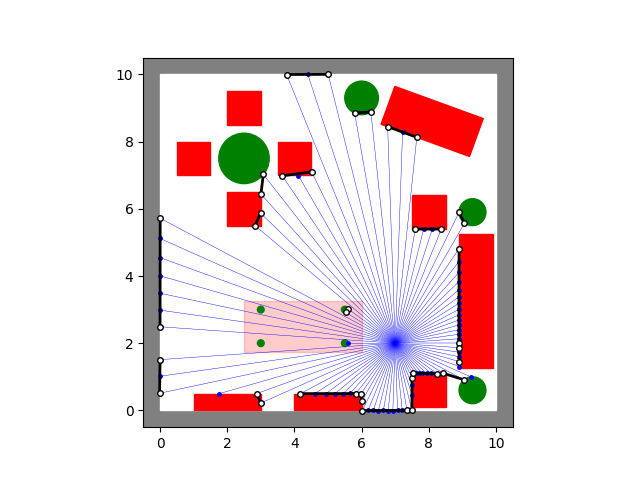
\includegraphics[width=0.80\textwidth]{img/rangeData_7_2_90.png} \\
	\hline
	Split-and-merge on \texttt{rangeData\_7\_2\_90} \\
\end{tabular}

\end{enumerate}

\section*{Problem 3: Linear Filtering}
\begin{enumerate}[label=(\roman*)]
\item % (i)

\begin{enumerate}
	\item
	\begin{equation}
	F = \begin{bmatrix}
	1 & 2 & 3 \\
	4 & 5 & 6 \\
	7 & 8 & 9
	\end{bmatrix}
	\end{equation}
	
	\item
	\begin{equation}
	F = \begin{bmatrix}
	2 & 3 & 0 \\
	5 & 6 & 0 \\
	8 & 9 & 0
	\end{bmatrix}
	\end{equation}
	
	\item
	This kernel is doing discrete difference (differentiation) of the image along the horizontal axis. It could be used to perform edge detection tasks.
	\begin{equation}
	F = \begin{bmatrix}
	2 & 2 & -2 \\
	5 & 2 & -5 \\
	8 & 2 & -8
	\end{bmatrix}
	\end{equation}
	
	\item
	This is an isotropic, normalized Gaussian kernel performing blurring on the image. It could be used to filter out high frequency information on either axis.
	\begin{equation}
	F = \frac{1}{16}\begin{bmatrix}
	21 & 36 & 33 \\
	52 & 80 & 68 \\
	57 & 84 & 69
	\end{bmatrix}
	\end{equation}
	
	
	
\end{enumerate}

\item % (ii)
I'm assuming that the question is alluding to the fact that performing correlation (or convolution) over an input of depth $d$ means we end up summing over $d$ individual correlations or convolutions performed on individual input channels.

This is saying that:

\begin{equation}
G(i,j) = \sum_{w} \Bigg( \sum_{u}\sum_{v} F_w(u,v) \cdot I_w(i+u,j+v) \Bigg)
\end{equation}
where $G(i,j)$ is a correlation operation at position $i,j$ of the image, and $F$ and $I$ are flattened vector representations of the kernel and current image patch (including padding) that we are operating over. Therefore, writing out the matrices explicitly:

\begin{equation}
G(i,j) = \sum_w
\begin{bmatrix}- & F_w^\mathsf{T}(u,v) & -\end{bmatrix}
\begin{bmatrix}| \\ I_w \\ |\end{bmatrix}
\end{equation}

which is of course equal to taking the dot product of $f$, which is a single big vector f of length $u\cdot v\cdot w$ with a single big vector $t(i,j)$ of length $u\cdot v\cdot w$ as expressed below:

\begin{equation}
G(i,j) = 
\begin{bmatrix}F_1^\mathsf{T} & \hdots & F_w^\mathsf{T}\end{bmatrix}
\begin{bmatrix}I_{1} \\ \vdots \\ I_{w}\end{bmatrix}
= f^\mathsf{T} t_{i,j}
\end{equation}

\item % (iii)
(code)

\item % (iv)
Naive implementation as above using a loop: Runtimes are 0.79, 1.36, 0.77, 0.80 seconds.

Vectorized implementation batching all image pixels: Runtimes are 0.13, 7.55, 0.12, 0.34 seconds.

\begin{enumerate}
\item To answer the first hint, no, G does not have to run sequentially pixel by pixel. For a mono-channel image, each individual patch could be flattened and stacked into a $u\cdot v$ by $h\cdot w$ array and processed in parallel.

\item To answer the second hint, the total number of addmul operations are $u \cdot v \cdot w \cdot h$ as we are applying a filter with a receptive field of $u$ by $v$ over a single-channel input of size $w$ by $h$. If the filter could be expressed as an outer product, the total cost would be $(u+v) \cdot w \cdot h$.

\item We could implement Winograd's minimal filtering algorithm that pre-computes intermediate values that depend only on kernel weights with the motivation of saving redundant computation.
\end{enumerate}

\item For large inputs, instead of direct convolution, we can first transform our input and kernel into the frequency domain via FFT (with suitable windowing), multiply the two signals, and then translate back into our original spatial domains via inverse DFT. This approach is an approximation, the accuracy of which depends on the Fourier window, but for large inputs, the performance gains are significant.

\item % (v)
We use the result that any $m\times n$ matrix of rank 1 could be expressed as a vector outer product $uv^\mathsf{T}$. This is because the column rank of any vector $u$ has to be equal to 1. To answer the question, if we know that a matrix is rank 1 and we simply wish to recover $u$ and $v^\mathsf{T}$, these correspond to the orthogonal matrices after performing SVD on the original matrix. Alternatively, $u$ could be any of its columns and $v$ is the single nonzero row left over after performing Gaussian elimination, up to a constant factor $k$.

Additionally, it is easy to see that for any $m\times n$ matrix of rank $r$, we can express it as a linear combination of $r$ matrices, which themselves could be expressed as the outer product of the linearly independent rows and columns of the original matrix. This is a generalization of the above result.

\item % (vi)
(code)

\item % (vii)
Convolution with a flipped filter in all its dimensions would produce the same output as correlation with an unmodified filter.

In other words,
\begin{equation}
\begin{aligned}
G(i,j) &= \sum_{u=1}^k\sum_{v=1}^l F(u,v)\cdot I(i-u, j-v) \\
&= \sum_{u=1}^k\sum_{v=1}^l F(k-u, l-v) \cdot I(i+u, j+v)
\end{aligned}
\end{equation}


\end{enumerate}

\section*{Problem 4: Template Matching}
\begin{enumerate}[label=(\roman*)]
\item % (i)
(code)

\item % (ii)
(code)

\item % (iii)
Taking a page from data augmentation, we can:

\begin{enumerate}
\item Alter the color of the filter to improve matching for color variations.
\item Perform rotation on the filter to account for rotated candidates.
\end{enumerate}

However, unlike a neural net implementation that learns and summarizes individual filters, our runtime would increase linearly with the number of filters we are applying on a given image. The upside is that this process is embarrasingly parallel.
	
\end{enumerate}


\section*{Problem 5: Stop Sign Detection and FSM in ROS}
\begin{enumerate}[label=(\roman*)]
\item % (i)
\texttt{supervisor.py} publishes two messages on the following prefixes:
\begin{enumerate}
	\item \texttt{/cmd\_pose}, type \texttt{geometry\_msgs.msg.Pose2D}
	\item \texttt{/cmd\_vel}, type \texttt{geometry\_msgs.msg.Twist}
\end{enumerate}

\item % (ii)
(code)

\item % (iii)
(code)

\item % (iv)
(code)

\item % (v)
null

\item % (vi)
\begin{tabular}[t]{l}
	\hline \\
	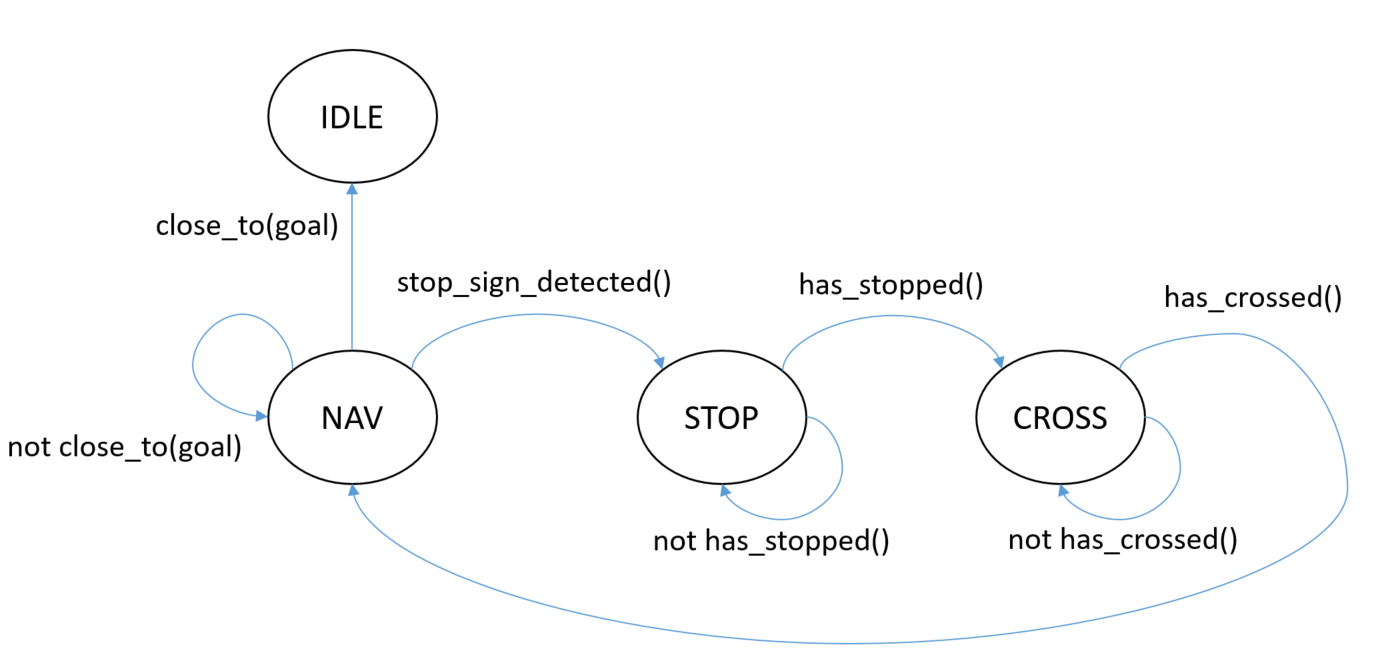
\includegraphics[width=0.7\textwidth]{img/state_machine.png} \\
	\hline
	FSM of \texttt{supervisor.py} \\
\end{tabular}

\item % (vii)
(code)

\item % (viii)
\begin{tabular}[t]{l}
	\hline \\
	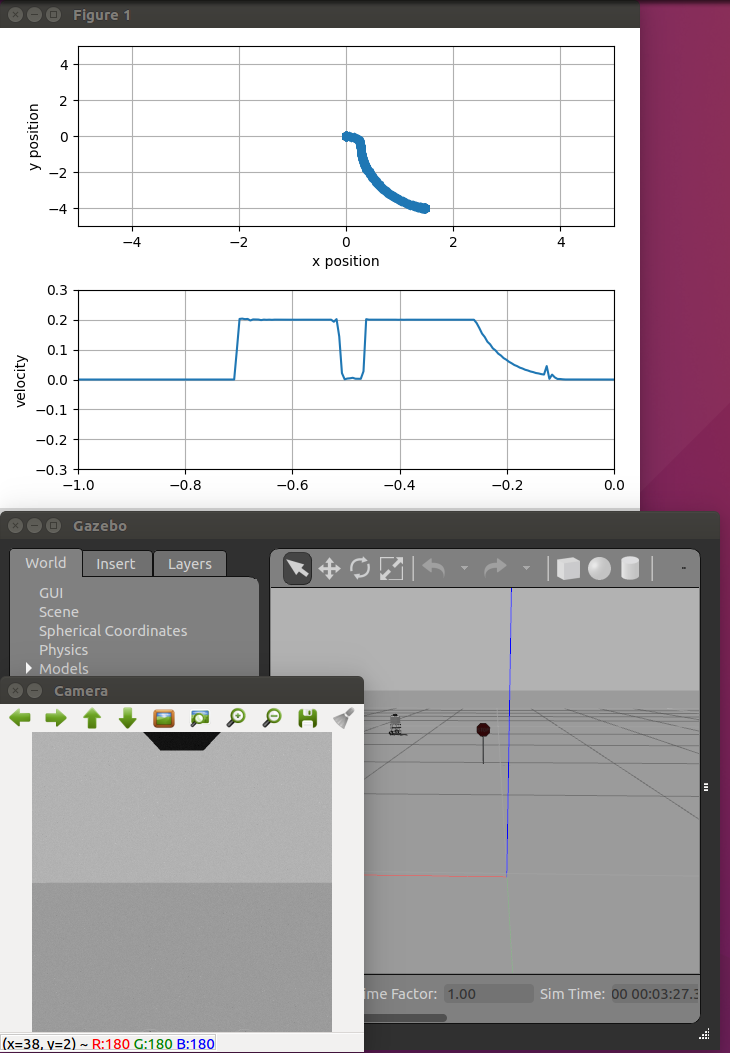
\includegraphics[width=0.7\textwidth]{img/vel_profile.png} \\
	\hline
	Velocity profile of Turtlebot model 'burger' under state machine policy. \\
\end{tabular}
	
\end{enumerate}

\section*{Extra Problem: Image Pyramids}
\begin{enumerate}[label=(\roman*)]
\item % (i)
(code)

\item % (ii)

We have lost high-frequency information as a by-product of our sampling process, specifically the signal or gradient between each adjacent pixel. Notice that some of the vertical lines are completely missing.
\begin{tabular}[t]{c}
	\hline \\
	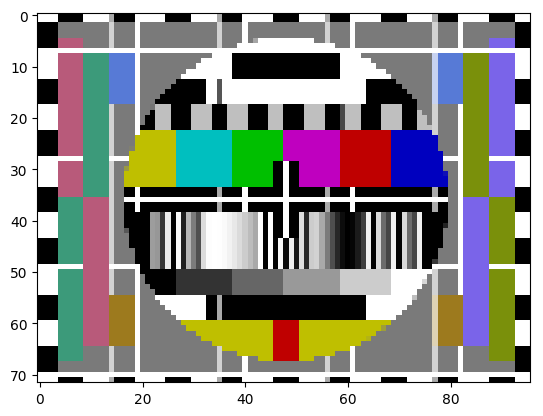
\includegraphics[width=0.7\textwidth]{img/test_card_eighthscale.png} \\
	1/8-sized image by discarding every other row and column 3 times. \\
	\hline
\end{tabular}

\item % (iii)
(code)

\item % (iv)
The Gaussian blur 'expanded' high frequency information along the x and y axes, so we preserve some component of those signals when sampling the image.

\begin{tabular}[t]{c}
	\hline \\
	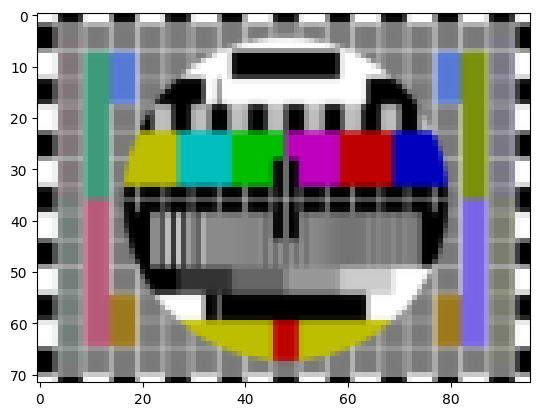
\includegraphics[width=0.7\textwidth]{img/test_card_blur_eighthscale.png} \\
	1/8-sized image with Gaussian blur (5x5 kernel) applied before discarding data. \\
	\hline
\end{tabular}

\pagebreak

\item % (v)
(code)

\item % (vi)
We have simply expanded each pixel by 8x along each dimension. To look at it another way, we have created 8x8 identical subpixels within each original pixel.

\begin{tabular}[t]{c}
	\hline \\
	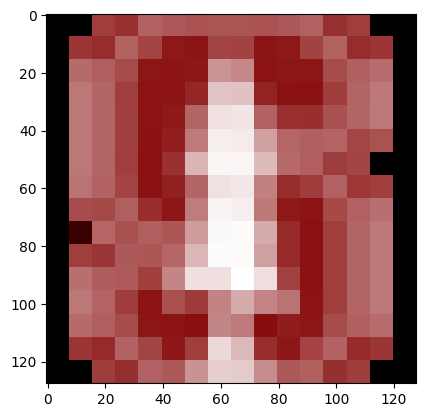
\includegraphics[width=0.5\textwidth]{img/favicon_upscale_8x.png} \\
	Image expanded 8 times without bilinear interpolation. \\
	\hline
\end{tabular}

\item % (vii)
(code).

\begin{tabular}[t]{l}
	\hline \\
	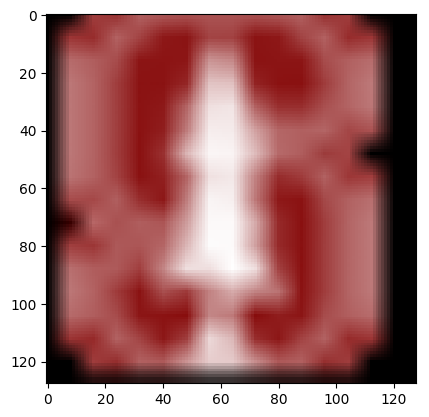
\includegraphics[width=0.5\textwidth]{img/favicon_bilinear_8x.png} \\
	Image expanded 8 times with bilinear interpolation. \\
	\hline
\end{tabular}

Comparing the images: the intensity differences between the pixel regions are less abrupt.

Informal explanation: I'm going to explain this in terms of a 2x upscaling. From the way we've expanded the image, and how OpenCV zero-pads the boundaries, we have 'islands' of pixels spread apart by exactly the same distance which we want to expand the image by. Also, normalization works out as a sanity check: The kernel for 2x2 upscaling sums to 4. 'Striding' or expanding the image as described for a 2x2 upscale effectively divides each region by 4. When viewed along these 'islands' of original pixel values, the tent function is doing discrete linear interpolation of values in between each island. Hence bilinear interpolation, because we have two axes $x$ and $y$. Without loss of generalization, this applies to any upscaling which is a factor or 2.

\item % (viii)
(code).

\begin{tabular}[t]{l}
	\hline \\
	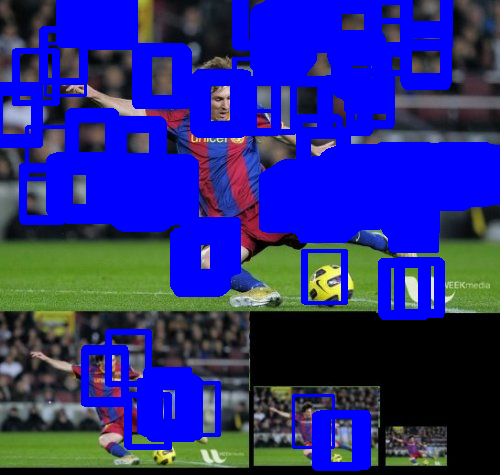
\includegraphics[width=1.0\textwidth]{img/image_detections.png} \\
	Bounding boxes with threshold = 0.82. \\
	This is the highest threshold at 2 significant figures that manages to match the second-smallest image. \\
	The precision / recall tradeoffs are severe. \\
	\hline
\end{tabular}

\pagebreak

\item % (xi)
The template only matches the original image, which is the second stop sign; it is not robust to intra-class variation.

\begin{tabular}[t]{l}
	\hline \\
	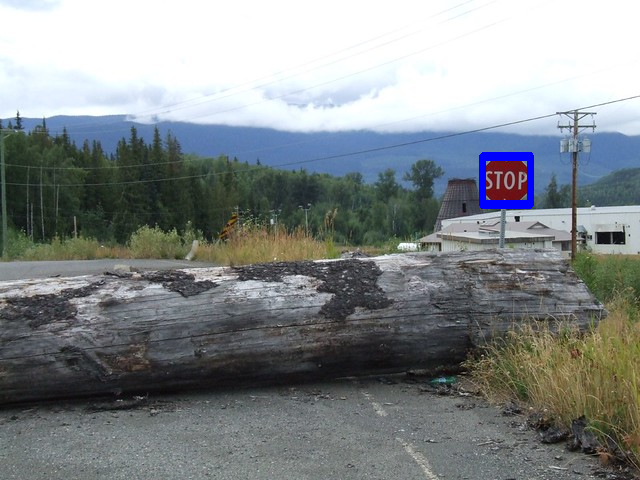
\includegraphics[width=1.0\textwidth]{img/stop2_detection.png} \\
	Bounding boxes at default threshold in pset. \\
	\hline
\end{tabular}

\end{enumerate}

\end{document}
